\documentclass[A4,svgnames,9pt,aspectratio=169]{beamer}
%% document options:
%% - aspectratio = { 43, 169, 1610 }
%% - utf8
%%

\usepackage[utf8]{inputenc}
\usepackage[T1]{fontenc}
\usepackage[french]{babel}
\usepackage{graphicx}
\usepackage{amsmath,amssymb,amsfonts}
\usepackage{booktabs}
\usepackage{xcolor}
\usepackage{tikz}

\hypersetup{
   allcolors=rouge_inria,
   pdfauthor   = {Louis Hauseux, Raphaël Antoine, Philippe Foucher, Pierre Charbonnier, Josiane Zerubia},
   pdftitle    = {Réunion Inria-Cerema : Sur les modèles de fondation},
   pdfsubject  = {Extraction de fissures multi-modale sans apprentissage},
   pdfkeywords = {Frangi, graph, betweenness centrality, multi-modal fusion}
}

% Commandes personnalisées
\newcommand{\eg}[0]{\textit{e.g., }}
\newcommand{\ie}[0]{\textit{i.e., }}
\newcommand{\etal}[0]{\textit{et al. }}
\newcommand{\norme}[1]{\left\lVert #1 \right\rVert}
\newcommand{\module}[1]{\left| #1 \right|}
\newcommand{\Frangi}[0]{\textsc{Frangi}}
\newcommand{\Hess}[0]{\mathcal{H}}
\newcommand{\nom}[1]{\textsc{#1}}

% Couleurs pour les courbes
\definecolor{myred}{HTML}{D62728}
\definecolor{mygreen}{HTML}{2CA02C}

\title[Réunion Inria-Cerema]{Réunion Inria-Cerema. \\ Sur les modèles de fondation.}
\subtitle{~}
\date[10/07/2026]{vendredi 10 juillet 2026}
\author[L. \textsc{Hauseux} \textit{et al.}]{%
  {\small Inria, éq. \textsc{Ayana} : Louis \textsc{Hauseux}, Josiane \textsc{Zerubia}} \\
  {\small Cerema, éq. \textsc{Endsum} : Raphaël \textsc{Antoine}, Philippe \textsc{Foucher}, Pierre \textsc{Charbonnier}}%
}
\institute{
  Inria, Université Côte d'Azur, Équipe Ayana, Sophia Antipolis, France \\
  Cerema, Équipe de recherche Endsum, France
}

\usetheme{inria}

% Personnalisation des notes de bas de page pour éviter qu'elles ne coupent la ligne du footer
\renewcommand{\footnoterule}{}
\setbeamertemplate{footnote}{%
  \parindent 0pt%
  \noindent%
  \raggedright%
  \hbox to 0.8em{\hfil\insertfootnotemark}%
  \insertfootnotetext\par%
  \vspace*{2.2ex}%
}

\begin{document}

\frame{\titlepage}

\renewcommand{\contentsname}{Sommaire}
\frame{\tocpage}

%%%%%%%%%%%%%%%%%%%%%%%%%%%%%%%%%%%%%%%%%%%%%%%%%%%%%%%
\section{Les modèles de fondation, le cas de CrackSAM}
\frame{\sectionpage}

\begin{frame}{Le Mécanisme d'Attention des \emph{Transformers}\footnotemark[1]}
    L'attention calcule la contribution de chaque élément $j$ à la représentation de l'élément $i$ :
    \begin{equation*}
        \mathbf{y}_i = \sum_{j} a_{ij} \mathbf{v}_j \quad \text{avec} \quad a_{ij} = \frac{\exp\left(\frac{\mathbf{q}_i \, {}^t \mathbf{k}_j}{\sqrt{d_k}}\right)}{\sum_{l} \exp\left(\frac{\mathbf{q}_i \, {}^t \mathbf{k}_l}{\sqrt{d_k}}\right)}
    \end{equation*}
    \vskip 1ex
    \begin{block}{Composantes de l'attention}
        \begin{itemize}
            \item \textbf{\emph{Queries} ($\mathbf{q}_i$) :} Requête de l'élément $i$ (ce qu'il cherche)
            \item \textbf{\emph{Keys} ($\mathbf{k}_j$) :} Clé de l'élément $j$ (ce qu'il propose)
            \item \textbf{\emph{Values} ($\mathbf{v}_j$) :} Valeur de l'élément $j$ (son contenu sémantique)
            \item \textbf{Facteur $\sqrt{d_k}$ et poids $a_{ij}$ :} Facteur d'échelle et score d'attention.
        \end{itemize}
    \end{block}
    \footnotetext[1]{\nom{Vaswani} \etal, \og Attention Is All You Need\fg{}, \textit{NeurIPS}, 2017.}
\end{frame}

\begin{frame}{\emph{Vision Transformers} (\emph{ViT}) : De l'Image aux Patchs\footnotemark[2]}
    L'architecture \emph{ViT} adapte les \emph{Transformers} au traitement d'images en découpant l'image en une séquence de morceaux :
    \vskip 1ex
    \begin{block}{Étapes clés de traitement}
        \begin{enumerate}
            \item \textbf{Découpage en patchs} : L'image est divisée en une grille de patchs de $16 \times 16$ pixels (qui jouent le rôle de mots).
            \item \textbf{Projection linéaire (\emph{Patch Embedding})} : Chaque patch est projeté vectoriellement dans un espace sémantique de dimension fixe.
            \item \textbf{\emph{Embeddings} de Position} : Ajout d'une coordonnée de position à chaque patch pour conserver la géométrie 2D de l'image.
            \item \textbf{Jeton sémantique global} : Ajout d'un jeton virtuel en début de séquence pour résumer toute l'image.
        \end{enumerate}
    \end{block}
    \footnotetext[2]{\nom{Dosovitskiy} \etal, \og An Image is Worth 16x16 Words: Transformers for Image Recognition at Scale\fg{}, \textit{ICLR}, 2021.}
\end{frame}

\begin{frame}{Modèles de Fondation \& \emph{Transformers}}
    \begin{columns}
        \begin{column}{0.5\textwidth}
            \begin{block}{Trois piliers des modèles de fondation}
                Un modèle unique pré-entraîné à grande échelle pour être adapté à de nombreuses tâches :
                \begin{itemize}
                    \item \textbf{\emph{Scale}} : taille du modèle (milliards de paramètres) et des données.
                    \item \textbf{Auto-supervision} : pré-entraînement autonome sans annotations.
                    \item \textbf{Adaptabilité (\emph{Fine tuning})} : socle commun réutilisable.
                \end{itemize}
            \end{block}
        \end{column}
        \begin{column}{0.48\textwidth}
            \begin{block}{Rôle des \emph{Transformers}}
                L'architecture \emph{Transformer} (\emph{ViT}, \emph{GPT}) domine largement ce domaine.
                \vskip 1ex
                \textbf{Avantages :}
                \begin{itemize}
                    \item Parallélisation massive (entraînement rapide sur \emph{GPU}).
                    \item Capacité de généralisation exceptionnelle.
                \end{itemize}
                \textbf{Limites :}
                \begin{itemize}
                    \item Complexité quadratique $O(N^2)$ sur la longueur des séquences.
                    \item Modèles complexes agissant comme des \og boîtes noires \fg{}.
                \end{itemize}
            \end{block}
        \end{column}
    \end{columns}
\end{frame}

\begin{frame}{SAM : \emph{Segment Anything Model}\footnotemark[3]}
    \begin{columns}
        \begin{column}{0.56\textwidth}
            \begin{block}{Architecture asymétrique}
                \begin{itemize}
                    \item \textbf{\emph{Image Encoder}} : Un grand \emph{ViT} (ViT-H, 637M paramètres) pré-entraîné (\emph{MAE}). Extrait un \emph{embedding} d'image de taille $64 \times 64$.
                    \item \textbf{\emph{Prompt Encoder}} : Module très léger. Encode les invites spatiales (points, boîtes via codage positionnel) ou textuelles (via \emph{CLIP}).
                    \item \textbf{\emph{Mask Decoder}} : Décodeur rapide par \emph{Transformer} bidirectionnel. Génère les masques en temps réel ($\sim 50$ ms).
                    \item \textbf{\emph{Dataset} SA-1B} : 11M d'images, 1,1 milliard de masques de haute qualité.
                \end{itemize}
            \end{block}
        \end{column}
        \begin{column}{0.41\textwidth}
            \centering
            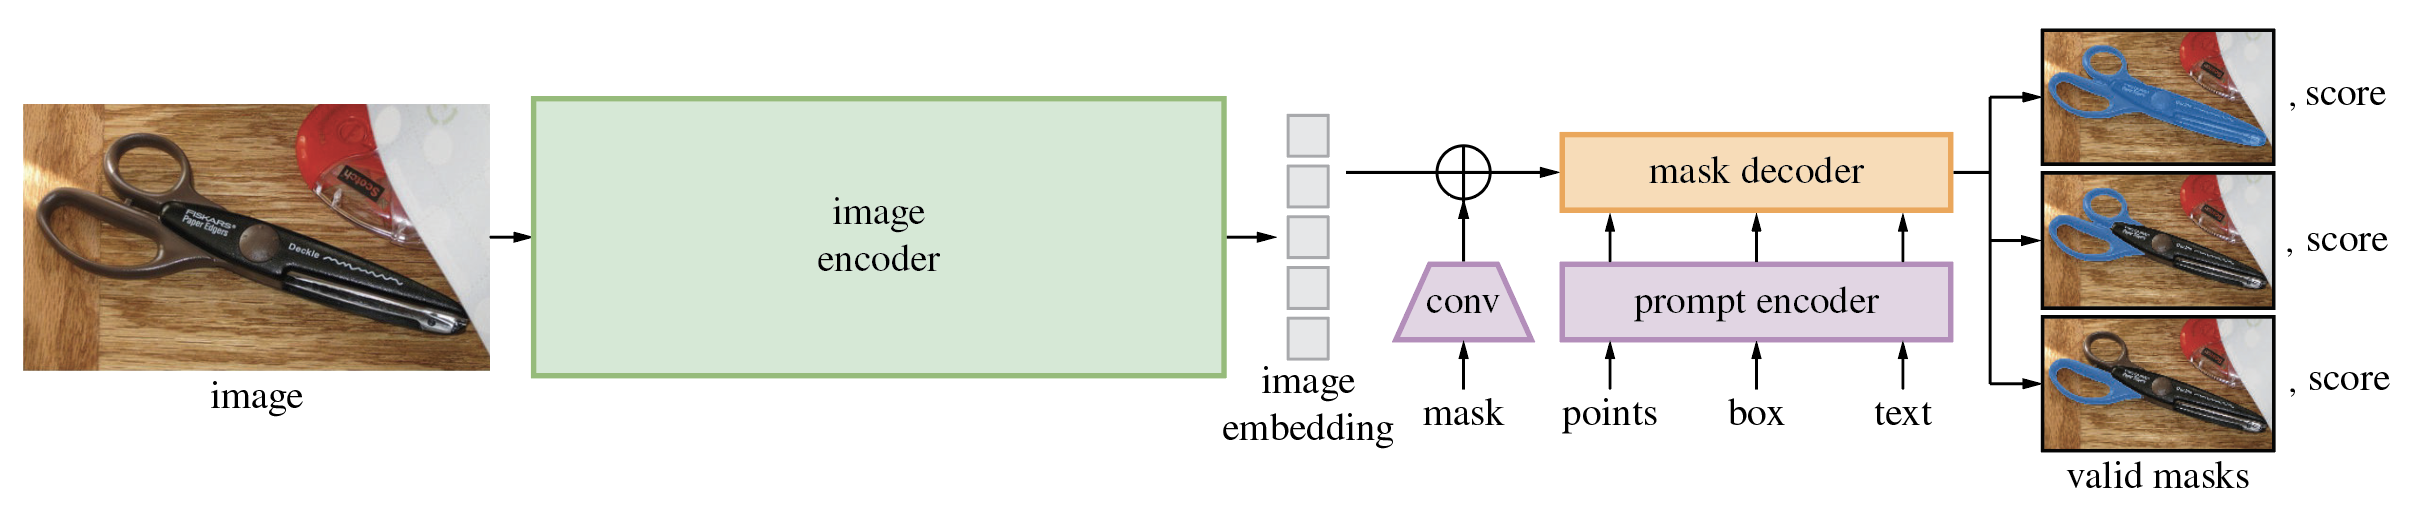
\includegraphics[width=\textwidth]{imgs/sam_model_diagram.png}
            \vskip 1ex
            {\scriptsize Schéma de SAM : Séparation stricte entre le calcul lourd (image) et le calcul rapide (invites).}
        \end{column}
    \end{columns}
    \footnotetext[3]{\nom{Kirillov} \etal, \og Segment Anything\fg{}, \textit{ICCV}, 2023. Code : \texttt{github.com/facebookresearch/segment-anything}}
\end{frame}

\begin{frame}{CrackSAM : \emph{Fine-Tuning} Efficace par \emph{LoRA}}
    \begin{block}{Difficultés de la détection de fissures}
        \begin{itemize}
            \item \textbf{Déséquilibre extrême} : Fissures couvrant une fraction infime des pixels.
            \item \textbf{Perturbations} : Présence d'ombres, de flous, d'humidité et textures rugueuses.
            \item \textbf{Changement de domaine} : Écart important avec le pré-entraînement généraliste.
        \end{itemize}
    \end{block}
    \vskip 1ex
    \begin{block}{Principe de la \emph{Low-Rank Adaptation} (\emph{LoRA})}
        On cherche les matrices $A$ et $B$ de petit rang $r$ à partir des poids gelés $W_0$ :
        \begin{equation*}
            W = W_0 + \Delta W \quad \text{avec} \quad \Delta W = B \cdot A
        \end{equation*}
        \textbf{Avantages :}
        \begin{itemize}
            \item Seules les matrices $A$ et $B$ sont entraînées ($W_0$ reste figée).
            \item Paramètres à entraîner divisés par 100 ($4,4$M contre $637$M).
        \end{itemize}
    \end{block}
\end{frame}

\begin{frame}{CrackSAM : Performances en \emph{Zéro-Shot}}
    \begin{columns}
        \begin{column}{0.54\textwidth}
            \begin{block}{Entraînement et Évaluation}
                \begin{itemize}
                    \item \textbf{Entraînement} : Ajustement fin (\emph{Fine-tuning}) sur le \emph{dataset} de \href{https://github.com/khanhha/crack_segmentation}{Khanhha} ($9\,603$ images de fissures).
                    \item \textbf{Évaluation} : Testé en \emph{zéro-shot} (sans réapprentissage) sur 3 benchmarks :
                        \begin{itemize}
                            \item \texttt{Road420} (routes, ombres, nuit).
                            \item \texttt{Facade390} (façades par drone, flou).
                            \item \href{https://github.com/Yuliang-Li/HrSegNet}{\texttt{Concrete3k}} ($3\,000$ images de béton).
                        \end{itemize}
                \end{itemize}
            \end{block}
            \begin{block}{Résultats et Distillation}
                \begin{itemize}
                    \item \textbf{SOTA pulvérisé} : Robustesse extrême au bruit (\emph{IoU} $+27\%$ à $+42\%$ sous fort flou face aux modèles classiques comme \emph{U-Net} ou \emph{SegFormer}).
                    \item \textbf{Distillation} : Possibilité de distiller vers un modèle élève (\emph{Student}) léger pour l'embarqué.
                \end{itemize}
            \end{block}
        \end{column}
        \begin{column}{0.42\textwidth}
            \centering
            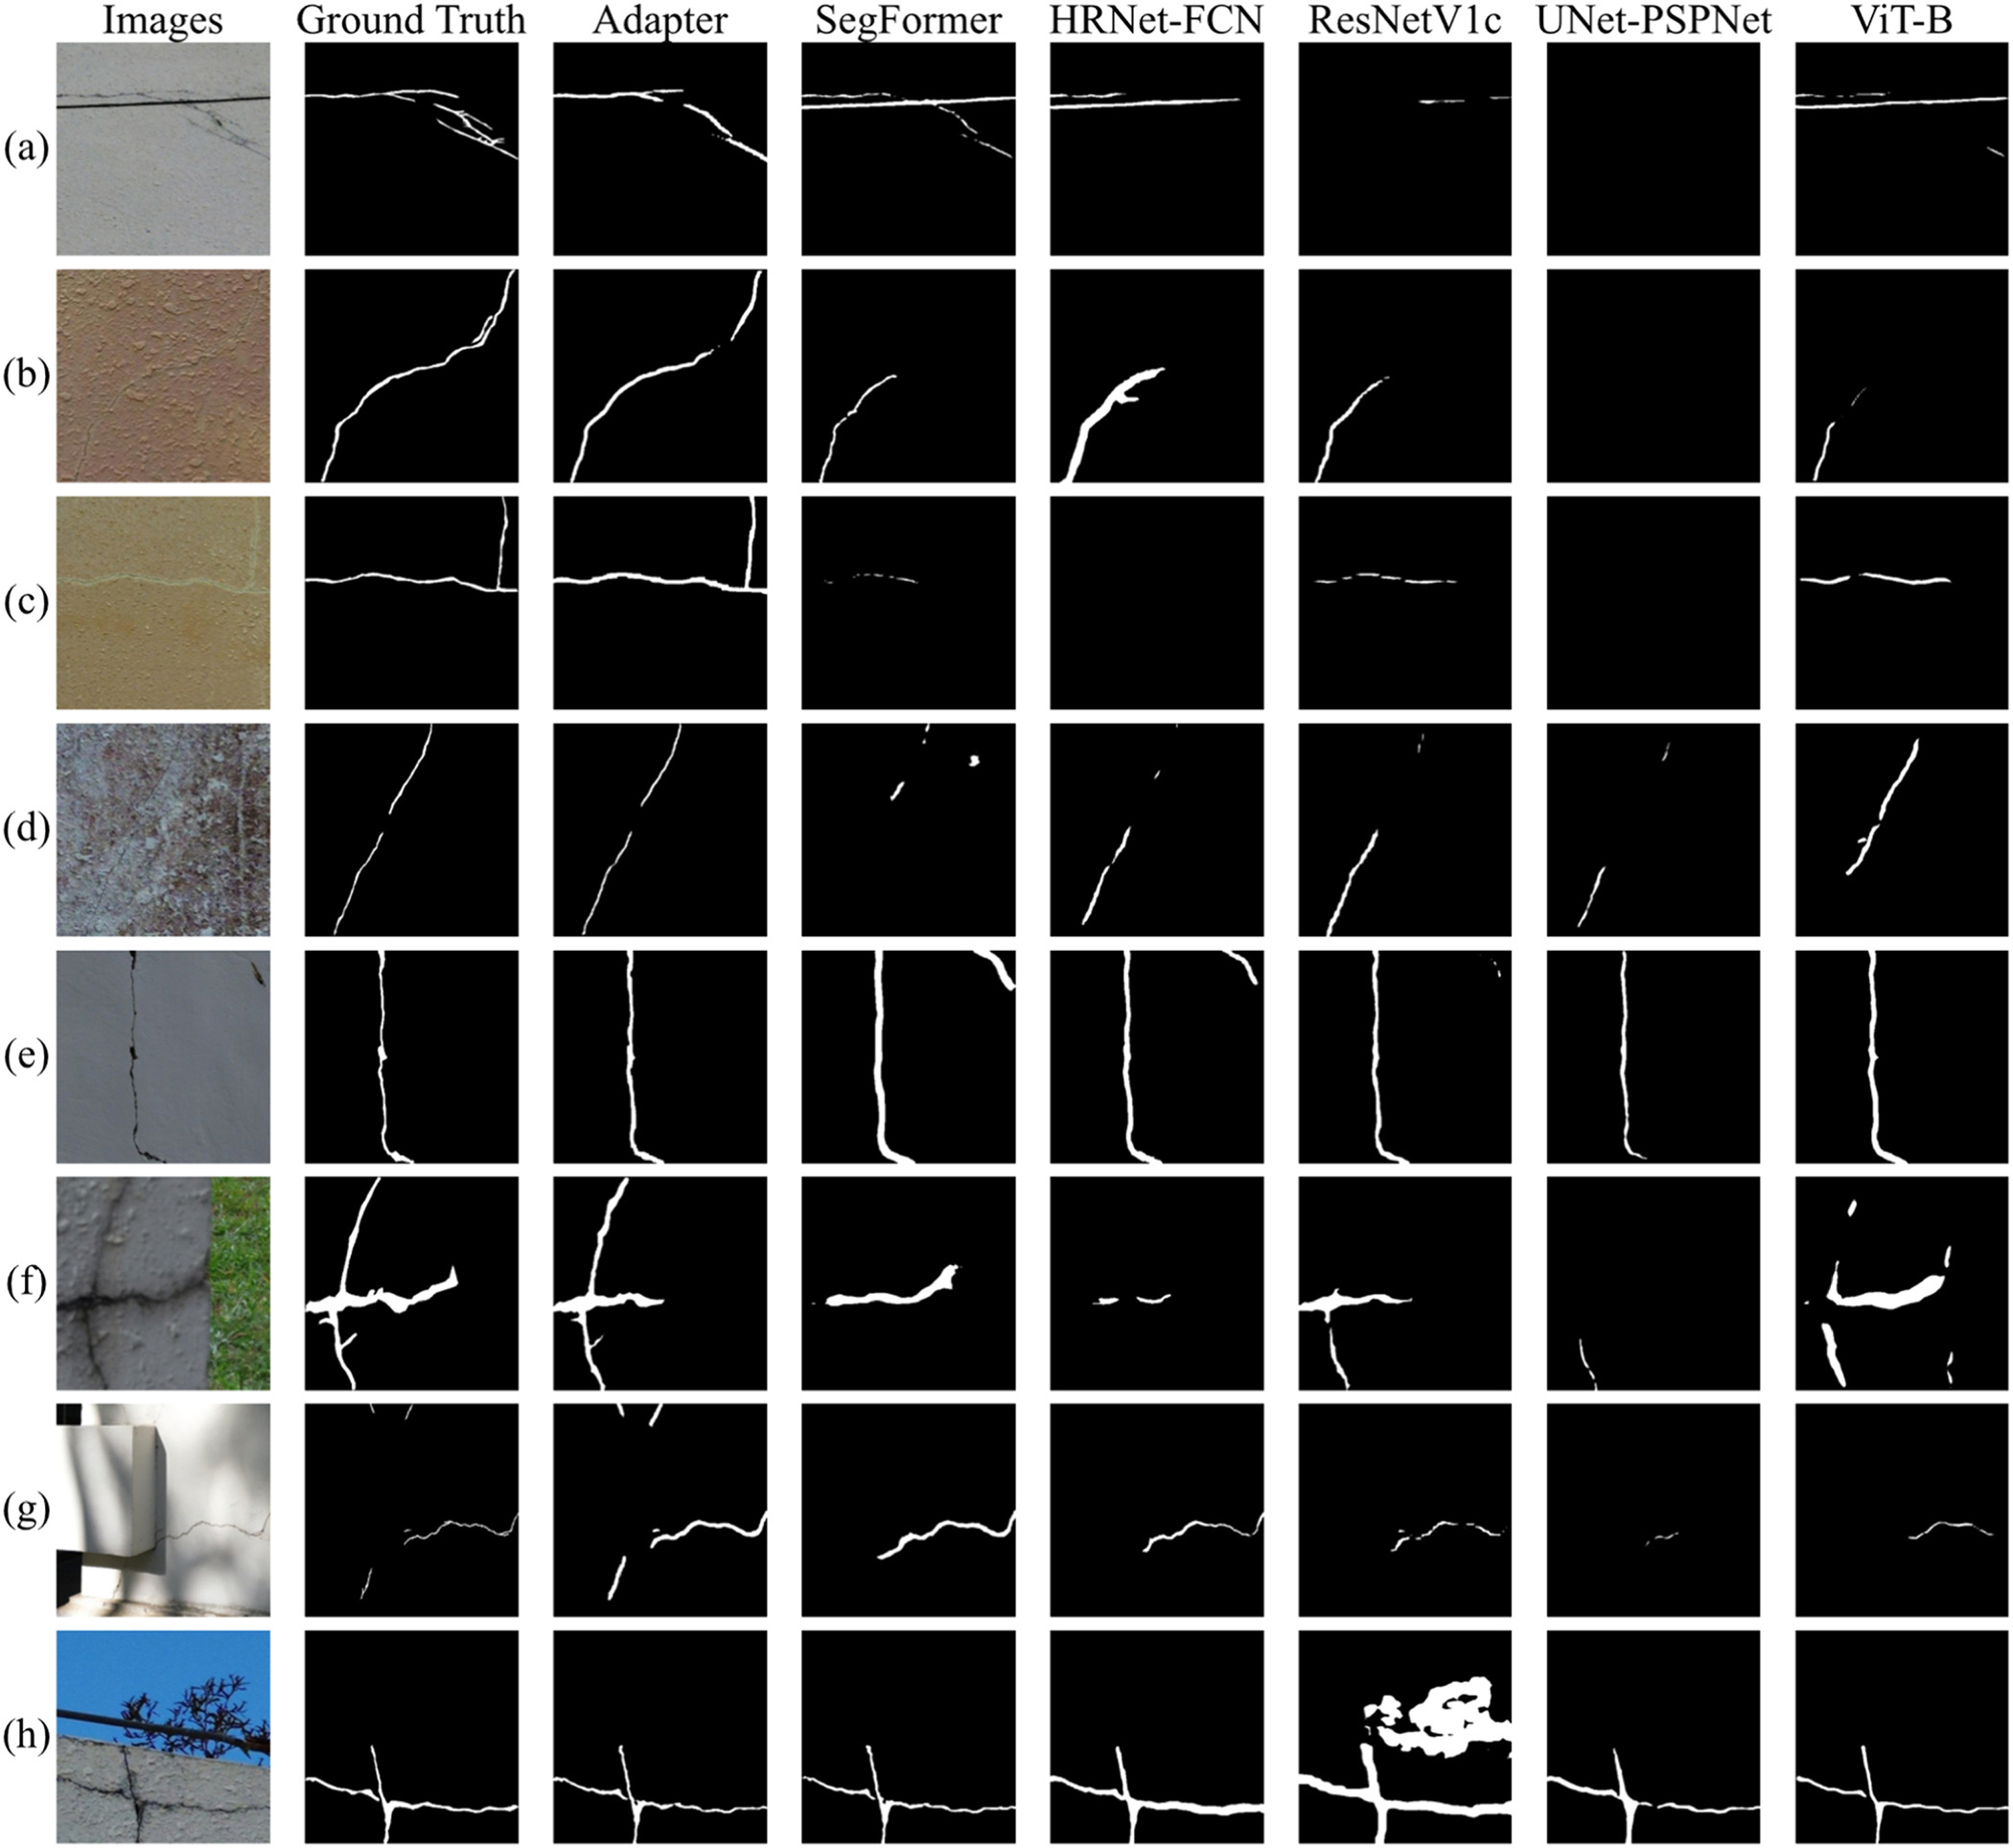
\includegraphics[width=\textwidth]{imgs/extracted_p11_0.jpg}
            \vskip 1ex
            {\scriptsize Comparaisons \emph{zéro-shot} de CrackSAM vs \emph{SOTA} sur \texttt{Road420}.}
        \end{column}
    \end{columns}
\end{frame}


\section{Résultats sur VT-GraF}
\frame{\sectionpage}

% Fissure 1
\begin{frame}{Fissure 1 : Entrées Multi-Modales}
    \begin{columns}
        \begin{column}{0.48\textwidth}
            \begin{block}{Entrée RGB}
                \centering
                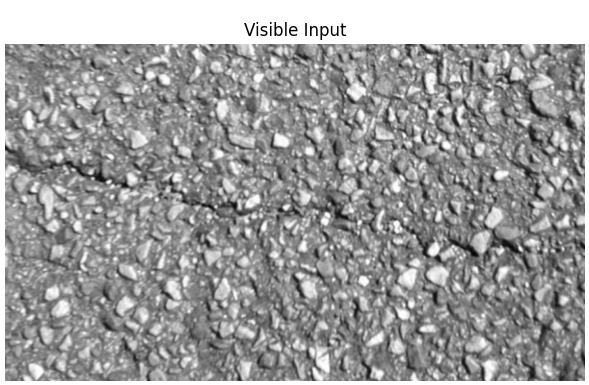
\includegraphics[width=\textwidth]{../results_images_cracksam/Fissure_1_rgb.png}
            \end{block}
        \end{column}
        \begin{column}{0.48\textwidth}
            \begin{block}{Modalité Thermique}
                \centering
                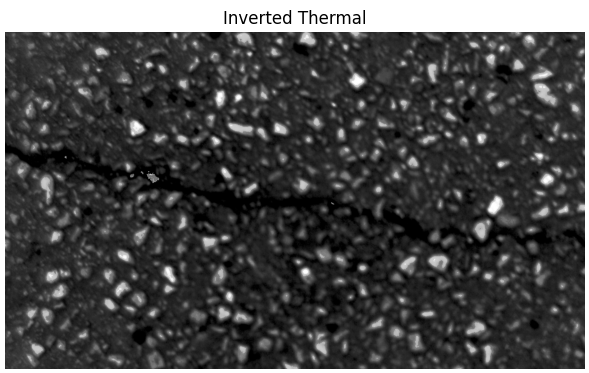
\includegraphics[width=\textwidth]{../results_images_cracksam/Fissure_1_thermal.png}
            \end{block}
        \end{column}
    \end{columns}
    \vskip 1ex
    {\scriptsize \textbf{Observations} : La fissure est peu visible sur l'image RGB mais ressort distinctement sur l'image thermique.}
\end{frame}

\begin{frame}{Fissure 1 : Extraction et Alignement}
    \begin{columns}
        \begin{column}{0.48\textwidth}
            \begin{block}{Similarité de Frangi}
                \centering
                
\includegraphics[width=\textwidth]{../results_images_cracksam/Fissure_1_frangi.png}
            \end{block}
        \end{column}
        \begin{column}{0.48\textwidth}
            \begin{block}{Superposition (Overlay)}
                \centering
                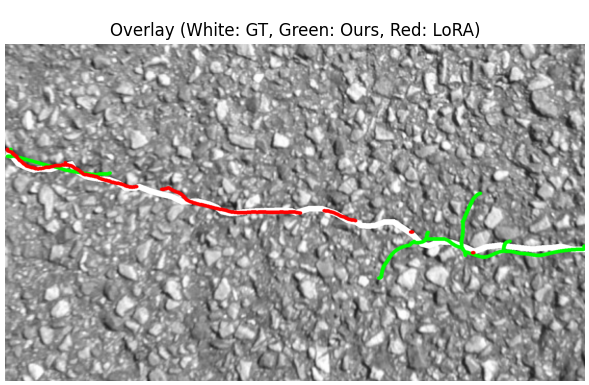
\includegraphics[width=\textwidth]{../results_images_cracksam/Fissure_1_overlay.png}
            \end{block}
        \end{column}
    \end{columns}
    \vskip 1ex
    {\scriptsize \textbf{Légende} : Vérité Terrain (\textbf{blanc}), Notre méthode (\textbf{vert}), et CrackSAM LoRA (\textbf{rouge}).}
\end{frame}

% Fissure 2
\begin{frame}{Fissure 2 : Entrées Multi-Modales}
    \begin{columns}
        \begin{column}{0.48\textwidth}
            \begin{block}{Entrée RGB}
                \centering
                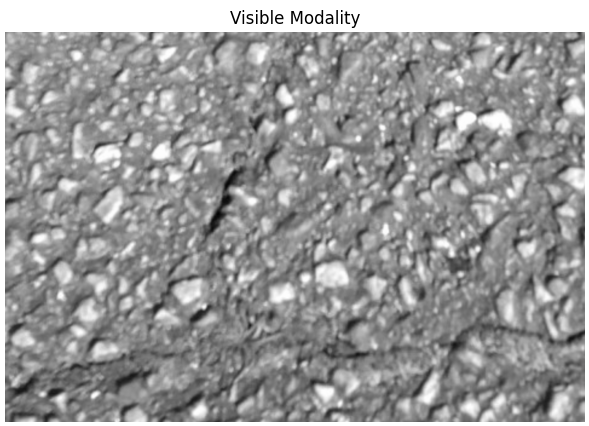
\includegraphics[width=\textwidth]{../results_images_cracksam/Fissure_2_rgb.png}
            \end{block}
        \end{column}
        \begin{column}{0.48\textwidth}
            \begin{block}{Modalité Thermique}
                \centering
                
\includegraphics[width=\textwidth]{../results_images_cracksam/Fissure_2_thermal.png}
            \end{block}
        \end{column}
    \end{columns}
    \vskip 1ex
    {\scriptsize \textbf{Observations} : Contraste RGB faible et présence de bruit de surface. Le signal thermique est plus net.}
\end{frame}

\begin{frame}{Fissure 2 : Extraction et Alignement}
    \begin{columns}
        \begin{column}{0.48\textwidth}
            \begin{block}{Similarité de Frangi}
                \centering
                
\includegraphics[width=\textwidth]{../results_images_cracksam/Fissure_2_frangi.png}
            \end{block}
        \end{column}
        \begin{column}{0.48\textwidth}
            \begin{block}{Superposition (Overlay)}
                \centering
                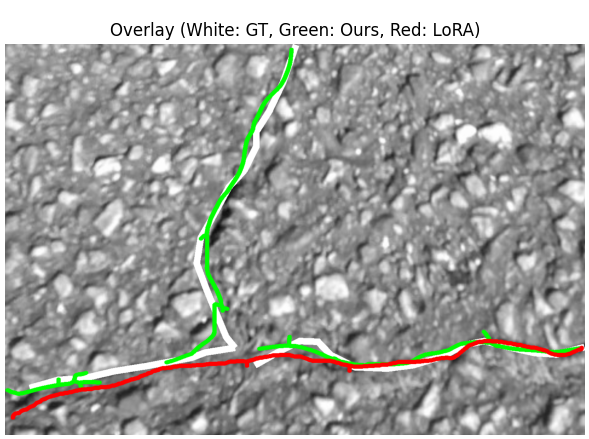
\includegraphics[width=\textwidth]{../results_images_cracksam/Fissure_2_overlay.png}
            \end{block}
        \end{column}
    \end{columns}
    \vskip 1ex
    {\scriptsize \textbf{Légende} : Vérité Terrain (\textbf{blanc}), Notre méthode (\textbf{vert}), et CrackSAM LoRA (\textbf{rouge}).}
\end{frame}

% Fissure 3
\begin{frame}{Fissure 3 : Entrées Multi-Modales}
    \begin{columns}
        \begin{column}{0.48\textwidth}
            \begin{block}{Entrée RGB}
                \centering
                
\includegraphics[width=\textwidth]{../results_images_cracksam/Fissure_3_rgb.png}
            \end{block}
        \end{column}
        \begin{column}{0.48\textwidth}
            \begin{block}{Modalité Thermique}
                \centering
                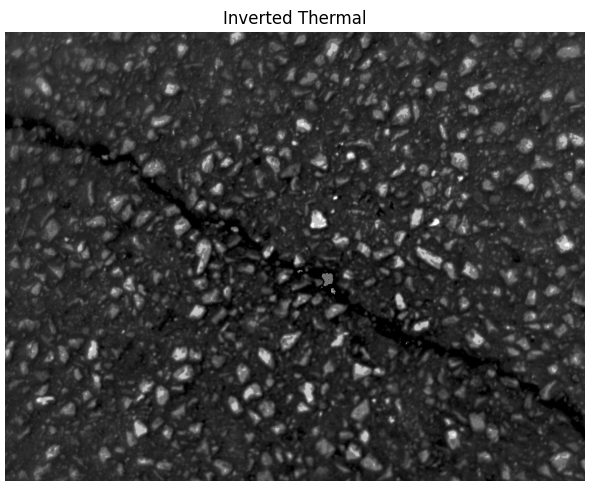
\includegraphics[width=\textwidth]{../results_images_cracksam/Fissure_3_thermal.png}
            \end{block}
        \end{column}
    \end{columns}
    \vskip 1ex
    {\scriptsize \textbf{Observations} : Fissure fine et sinueuse. Le canal thermique confirme le tracé topologique.}
\end{frame}

\begin{frame}{Fissure 3 : Extraction et Alignement}
    \begin{columns}
        \begin{column}{0.48\textwidth}
            \begin{block}{Similarité de Frangi}
                \centering
                
\includegraphics[width=\textwidth]{../results_images_cracksam/Fissure_3_frangi.png}
            \end{block}
        \end{column}
        \begin{column}{0.48\textwidth}
            \begin{block}{Superposition (Overlay)}
                \centering
                
\includegraphics[width=\textwidth]{../results_images_cracksam/Fissure_3_overlay.png}
            \end{block}
        \end{column}
    \end{columns}
    \vskip 1ex
    {\scriptsize \textbf{Légende} : Vérité Terrain (\textbf{blanc}), Notre méthode (\textbf{vert}), et CrackSAM LoRA (\textbf{rouge}).}
\end{frame}

% Fissure 4
\begin{frame}{Fissure 4 : Entrées Multi-Modales}
    \begin{columns}
        \begin{column}{0.48\textwidth}
            \begin{block}{Entrée RGB}
                \centering
                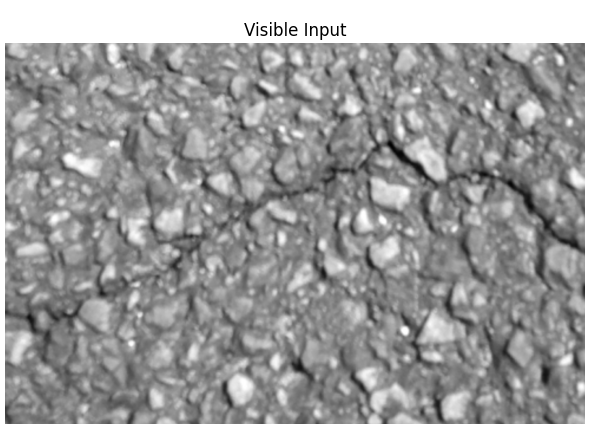
\includegraphics[width=\textwidth]{../results_images_cracksam/Fissure_4_rgb.png}
            \end{block}
        \end{column}
        \begin{column}{0.48\textwidth}
            \begin{block}{Modalité Thermique}
                \centering
                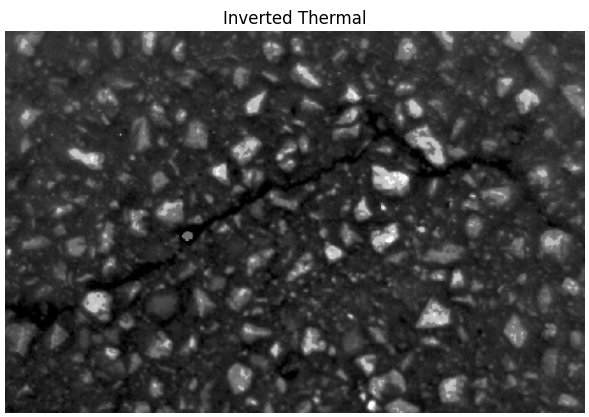
\includegraphics[width=\textwidth]{../results_images_cracksam/Fissure_4_thermal.png}
            \end{block}
        \end{column}
    \end{columns}
    \vskip 1ex
    {\scriptsize \textbf{Observations} : Forte intensité lumineuse ambiante masquant la fissure en RGB. Température contrastée en infrarouge.}
\end{frame}

\begin{frame}{Fissure 4 : Extraction et Alignement}
    \begin{columns}
        \begin{column}{0.48\textwidth}
            \begin{block}{Similarité de Frangi}
                \centering
                
\includegraphics[width=\textwidth]{../results_images_cracksam/Fissure_4_frangi.png}
            \end{block}
        \end{column}
        \begin{column}{0.48\textwidth}
            \begin{block}{Superposition (Overlay)}
                \centering
                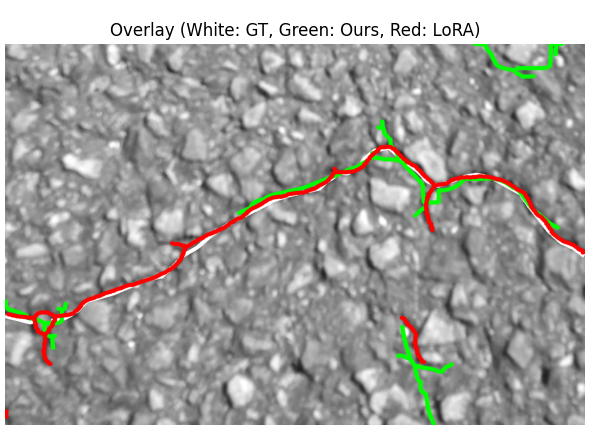
\includegraphics[width=\textwidth]{../results_images_cracksam/Fissure_4_overlay.png}
            \end{block}
        \end{column}
    \end{columns}
    \vskip 1ex
    {\scriptsize \textbf{Légende} : Vérité Terrain (\textbf{blanc}), Notre méthode (\textbf{vert}), et CrackSAM LoRA (\textbf{rouge}).}
\end{frame}

% Fissure 5
\begin{frame}{Fissure 5 : Entrées Multi-Modales}
    \begin{columns}
        \begin{column}{0.48\textwidth}
            \begin{block}{Entrée RGB}
                \centering
                
\includegraphics[width=\textwidth]{../results_images_cracksam/Fissure_5_rgb.png}
            \end{block}
        \end{column}
        \begin{column}{0.48\textwidth}
            \begin{block}{Modalité Thermique}
                \centering
                
\includegraphics[width=\textwidth]{../results_images_cracksam/Fissure_5_thermal.png}
            \end{block}
        \end{column}
    \end{columns}
    \vskip 1ex
    {\scriptsize \textbf{Observations} : Fissure complexe avec embranchements. La modalité thermique guide l'extraction géométrique.}
\end{frame}

\begin{frame}{Fissure 5 : Extraction et Alignement}
    \begin{columns}
        \begin{column}{0.48\textwidth}
            \begin{block}{Similarité de Frangi}
                \centering
                
\includegraphics[width=\textwidth]{../results_images_cracksam/Fissure_5_frangi.png}
            \end{block}
        \end{column}
        \begin{column}{0.48\textwidth}
            \begin{block}{Superposition (Overlay)}
                \centering
                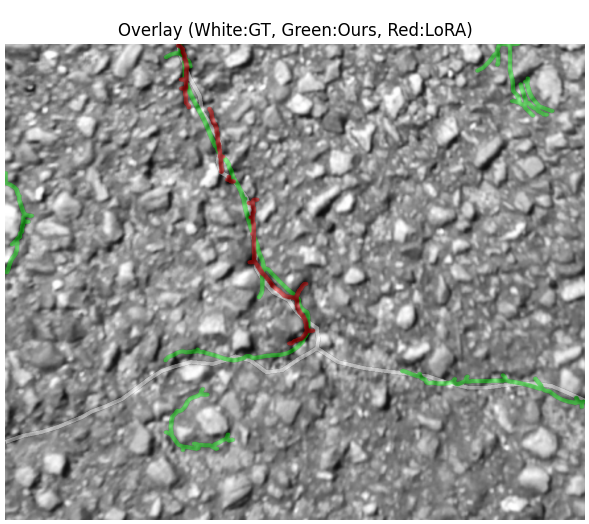
\includegraphics[width=\textwidth]{../results_images_cracksam/Fissure_5_overlay.png}
            \end{block}
        \end{column}
    \end{columns}
    \vskip 1ex
    {\scriptsize \textbf{Légende} : Vérité Terrain (\textbf{blanc}), Notre méthode (\textbf{vert}), et CrackSAM LoRA (\textbf{rouge}).}
\end{frame}


\frame{\merci}

\end{document}
